\documentclass{article}

\input{../../../preambule}
\usepackage{dsfont}

\title{Rapport de Projet de Fin d'Étude : Étude de la propagation d'un pathogène dans un blé.}
\author{Alexandre \bsc{Vieira}}
\date{\today}

\hypersetup{colorlinks=true, urlcolor=bleu, linkcolor=red}

\begin{document}

\maketitle
\tableofcontents

\newpage

\section*{Introduction}

\section{Modèle mathématique étudié}
Les modèles mathématiques présentés ici viennent tous de \cite{KotMedlock03}. 
\subsection{Différents modèles}
Pour décrire mathématiquement les invasions épidémiques, de nombreux modèles ont été décrit. Le plus simple qu'on puisse trouver est le modèle SI, comme présenté dans \cite{daley2001epidemic}. En notant $S(t)\geq 0$ les individus suceptibles et $I(t)\geq 0$ les individus infectés, où $t$ modélise dans chaque cas le temps, ce modèle s'écrit :
\begin{equation} \label{eq1}
\begin{array}{c c c}
	\frac{dS}{dt}&=&-\beta SI\\
	\frac{dI}{dt}&=&\beta SI
\end{array}
\end{equation}
où $\beta\geq 0$ est le taux de transmission. Ce genre de système se comprend aisément : l'évolution des deux classes est proportionnel au produit du nombre d'individu dans chaque classe, et les deux évolutions sont opposées.\\
Dans ce genre de système, on ne considère ni naissance ni mort. Ainsi, la taille de la popuation $N=S+I$ est constant. On transforme ainsi l'équation (\ref{eq1}), qui devient :
\begin{equation}\label{eqSI}
	\frac{dI}{dt}=\beta I(N-I)
\end{equation}
Cependant, la solution $I(t)$ peut être un peu plus complète en ajoutant une dimension spatiale au taux d'infectés.

\bigskip
Cette modélisation a été dérivé par Mollison \cite{mollison1972}. Dans celui-ci, les contacts entre les individus sont distribués spatiallement (comme des spores voyageant dans l'air par exemple). À chaque point $x$ d'un domaine $\Omega$, l'évolution dépendra encore une fois du produit entre le nombre de suceptibles et une moyenne ponderée des infectés.\\
On note cette fois $I(x,t)\geq 0$ la densité d'infectés au point $x$ à l'instant $t$. On considère comme auparavant la population totale $N$ constante, et par analogie au modèle (\ref{eqSI}), on a :
\begin{equation} \label{eqKot}
	\derPar{I}{t}(x,t)=\beta(x)(N-I(x,t))\int_{\mathbb{R}}k(x,y)I(y,t) dy
\end{equation}
Le noyau $k(x,y)$ est une densité pour la proportion d'infectés à $y$ qui peuvent contaminer des individus au point $x$. Ce noyau est une fonction positive, intégrable où \[\int_\Omega k(x,y) dx=1\]
On considère, pour le reste de notre étude, que ce noyau est de type convolutif, ie $k(x,y)=k(u)$ et qu'il admet une fonction génératrice des moments :
	\[M(\theta)=\int_{\mathbb{R}} k(y)e^{\theta y} dy\]
Un bon exemple est le noyau gaussien, que nous prendrons pour tout le reste de l'étude :
\begin{equation}\label{noyGau}
	k(x)=\frac{1}{\sqrt{2\alpha\pi}} \exp\left(-\frac{x^2}{2\sigma^2} \right)
\end{equation}

\bigskip
Il existe également d'autres individus, comme le modèle d'infectieux distribués, où on modélise également le mouvement de populations dans l'espace. Il est donné par :
\begin{equation}
	\derPar{I}{t}(x,t)=\beta(x)(N-I(x,t))-DI(x,t)+D\int_{\mathbb{R}}k(x,y)I(y,t) dy
\end{equation}
où $D$ est le taux auquel les individus change de position dans $\Omega$. Nous ne nous intéresserons pas à ce genre de modèle et nous nous concentrerons uniquement sur le modèle (\ref{eqKot})

\subsection{Étude de la vitesse de propagation}
Medlock \cite{KotMedlock03} a montré que la vitesse de propagation de la solution du modèle (\ref{eqKot}) $I_n$ est bornée par la solution du modèle linéaire $I_0$, linéarisé autour du point d'équilibre $I=0$ :
\begin{equation}\label{modLin}
\derPar{I}{t}=\beta(x)N\int_{\mathbb{R}}k(x,y)I(y,t) dt
\end{equation}
\[I_n(x,t)\leq I_0(x,t)\]
Si de plus, la condition initiale est bornée par une exponentielle \[I_0(x,0)\leq Ae^{-\theta x}\] on aura une borne supérieure pour la vitesse de propagation :
\begin{equation}\label{bornSup}
	I_0(x,t)\leq Ae^{\theta'(x-c(\theta')t)}\ \forall \theta'\leq \theta
\end{equation}
Mollison \cite{mollison1991dependence} avance la conjecture suivante : la vitesse de propagation du modèle non linéaire sera toujours la même que celle de son modèle linéaire, sous les hypothèses suivantes :
\begin{itemize}
	\item Le taux de croissance des individus sur un site ne croit pas avec le nombre d'individus présent sur le site
	\item L'influence des individus lointains est négligeable.
\end{itemize}
Sous cette conjecture, on peut facilement calculer la vitesse de propagation du front : en prenant $I$ sous la forme d'une onde propagatrice de vitesse $c$ :
	\[I(x,t)=Ae^{-\theta(x-ct)}\]
et en réinjectant cela dans (\ref{eqKot}), on obtient :
	\[c=\beta(x)\frac{M(\theta)}{\theta}\]
où $M(\theta)$ est la fonction génératrice des moments :
Pour avoir la borne supérieure, on doit prendre l'infimum :
\begin{equation}\label{bornVit}
	c=\beta(x)\inf_{\theta>0}\frac{M(\theta)}{\theta}
\end{equation}

\subsection{Étude de la forme du front d'onde}
On se limite ici à un front d'onde sur la droite réelle vérifiant l'équation (\ref{eqKot}) et se propageant vers $+\infty$.\\
Le front d'onde connecte les deux points d'équilibre $I=0$ et $I=1$. Par un raisonnement par perturbations, Medlock \cite{KotMedlock03} propose une approximation de la forme de la solution de l'onde propagatrice.\\
On commence par définir $z=x-ct$ avec $c>0$ et on pose $I(x,t)=I(z)$. Ainsi, (\ref{eqKot}) devient :
\begin{equation}\label{eq39}
	cI'(z)+\beta(1-I(z))\int_{\mathbb{R}}k(z-y)I(y)dy=0
\end{equation}
On pose également $\xi=\frac{z}{c}$ et $g(\xi)=I(z)$. En réintroduisant cela dans l'intégrale, et en faisant un développement limité, on obtient :
\begin{eqnarray*}
	\int_{\mathbb{R}}k(u)I(z-u)du&=&\int_{\mathbb{R}} k(u)g\left(\xi-\frac{u}{c}\right)\\
				&=& \int_{\mathbb{R}} k(u)\left( g(\xi)-\frac{u}{c} g'(\xi)+O\left(\frac{1}{c^2}\right)\right) du\\
				&=& g(\xi) -\frac{M'(0)}{c} g'(\xi) +O\left(\frac{1}{c^2}\right)
\end{eqnarray*}
Ainsi, (\ref{eq39}) devient :
\begin{equation}\label{eq40}
	g'(\xi)=-\beta(1-g(\xi))\left( g(\xi)-\frac{M'(0)}{c}g'(\xi)+O\left(\frac{1}{c^2}\right)\right)
\end{equation}

vérifiant
\begin{equation}\label{condBor}
	g(-\infty)=1,\ g(+\infty)=0,\ g(0)=\frac{1}{2}
\end{equation}

On note à présent \[g(\xi)=g_0(\xi)+\frac{1}{c} g_1(\xi)+O\left(\frac{1}{c^2}\right)\]
En réintroduisant cela dans (\ref{eq40}) et en identifiant les puissances de $\frac{1}{c}$, on obtient :
\begin{equation}\label{eqPert}
\begin{array}{r c l}
	g_0'(\xi)&=&-\beta g_0(\xi)(1-g_0(\xi))\\
	g_1'(\xi)&=&-\beta g_1(\xi)(1-2g_0(\xi))+\beta M'(0)g_0'(\xi)(1-g_0(\xi))
\end{array}
\end{equation}

satisfaisant :
\begin{equation}
\begin{array}{c}
	g_0(-\infty)=1,\ g_0(+\infty)=0,\ g_0(0)=\frac{1}{2}\\
	g_1(-\infty)=0,\ g_1(+\infty)=0,\ g_1(0)=0
\end{array}
\end{equation}

La solution à ces équations est :
\begin{equation}
\begin{array}{r c l}
	g_0(\xi)&=&\frac{1}{1+\exp(\beta\xi)}\\
	g_1(\xi)&=&-\beta M'(0)\frac{\exp(\beta \xi)}{(1+\exp(\beta\xi))^2}\ln\left(\frac{1+\exp(\beta\xi)}{2}\right)
\end{array}
\end{equation}

Et donc :
\[I(z)=g\left(\frac{z}{c}\right)=\frac{1}{1+\exp\left(\beta\frac{z}{c}\right)}-\beta M'(0)\frac{\exp\left(\beta \frac{z}{c}\right)}{\left(1+\exp\left(\beta\frac{z}{c}\right)\right)^2}\ln\left(\frac{1+\exp\left(\beta\frac{z}{c}\right)}{2}\right)+O\left(\frac{1}{c^2}\right)\]
Cependant, comme $M'(0)=0$ pour des noyaux symétriques, on se retrouve rapidement limité. Medlock a poussé le raisonnement à des ordres supérieurs, ce qui donne l'expression suivante :
\[I(z)=\frac{1}{1+\exp\left(\beta\frac{z}{c}\right)}-\frac{\beta^2 M''(0)}{2c^2}\frac{\exp\left(\beta \frac{z}{c}\right)}{\left(1+\exp\left(\beta\frac{z}{c}\right)\right)^2}\left[\frac{1-\exp\left(\beta\frac{z}{c}\right)}{1+\exp\left(\beta\frac{z}{c}\right)}+\ln\left(\frac{1+\exp\left(\beta\frac{z}{c}\right)}{2}\right)\right]+O\left(\frac{1}{c^4}\right)\]
La figure \ref{plotShape} montre différents tracés de cette approximation à l'ordre 0.

\begin{figure}[!h]
	\centering
	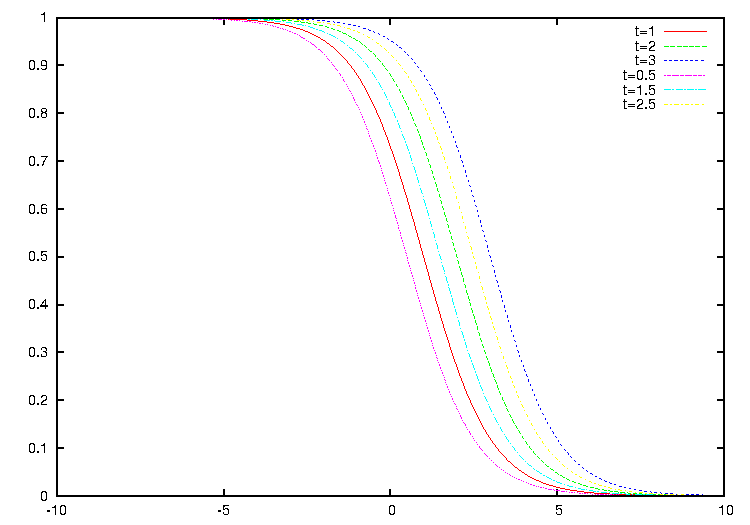
\includegraphics[scale=1]{img/plotShape.pdf}
\caption{Forme approchée du front à l'ordre 0 : $\beta=1$, $c=1$}
\label{plotShape}
\end{figure}

\section{Simulation numérique}
\subsection{Simplification de l'équation}
Afin d'étudier notre problème, l'équation (\ref{eqKot}) a été approchée par un autre modèle. Comme Medlock l'a montré \cite{KotMedlock03}, le modèle (\ref{eqKot}) a une vitesse bornée par le modèle linéaire :
On suppose, et nous garderons cette hypothèse dans toute la suite, que nous avons un noyau convolutif symétrique par rapport à l'origine. On peut prendre pour cela un noyau gaussien par exemple (et c'est celui que nous garderons par la suite) :
\[k(x,y)=\frac{1}{\sqrt{\alpha^2\pi}}\exp\left(\frac{(x-y)^2}{2\alpha^2}\right)\]
Formellement, on écrit le taux d'infectés $I$ sous la forme d'une série sous l'intégrale :
\begin{eqnarray*}
\frac{\partial I}{\partial t}(x,t) &=& \beta(x)N\int_{\mathbb{R}} k(y)I(x-y,t)dy\\
				&=&\beta(x)N\int_{\mathbb{R}} k(y)\sum_{n=0}^{+\infty} \frac{1}{n!} \frac{\partial^n I}{\partial x^n}(x,t)(-y)^n dy\\
				&=&\beta(x)N\sum_{n=0}^{+\infty} \frac{(-1)^n}{n!} \frac{\partial^n I}{\partial x^n}(x,t) \underbrace{\int_{\mathbb{R}} y^n k(y) dy}_{=\mu_n}\\
				&=&\beta(x)N\sum_{n=0}^{+\infty} \frac{(-1)^n\mu_n}{n!} \frac{\partial^n I}{\partial x^n}(x,t)
\end{eqnarray*}
Les $\mu_i$ étant les moments d'ordre $i$ du noyau. On normalise notre équation pour avoir $N=1$, et on garde en mémoire que pour la plupart des noyaux (dont le noyau gaussien), le moment d'ordre 0 vaut 1 et le moment d'ordre 1 s'annule. En gardant seulement les trois premiers termes, on a ainsi :
\begin{equation}\label{approx}
	\derPar{I}{t}(x,t)=\beta(x)\left(I(x,t)+\frac{\mu_2}{2}\derPar{{}^2I}{x^2}\right)
\end{equation}
Il reste ainsi à voir en quel sens cette équation approxime le modèle de départ.

\subsection{Cadre de la simulation}
Pour nos simluations, nous nous sommes placé sur un carré 2D maillé avec un pas constant. Ce carré représente un champ contenant deux variétés différentes, dont nous supposons que la sensibilité au pathogène est constante par rapport à la variété. Ainsi, notre $\beta$ dépendra uniquement de la variété présente en $x$, ce qui donnera une fonction constante par morceaux sur notre domaine.\\
Nous avons choisi deux cas pour la répartition de nos variétés : en bande ou en damier. La largeur de chaque bande (ou de chaque patch) restait modulable.\\
On a également besoin d'une solution initiale : nous avons choisi une répartition gausienne, centrée au milieu du domaine.
Pour nos simulations numériques, les dérivées en espace étaient calculées par un schéma du type volumes finis, et la résolution en temps était faite grâce à la méthode des lignes, utilisant un schéma de Runge-Kutta d'ordre 4.\\
\paragraph{Petit aparté sur la méthode des lignes :} La méthode des lignes sert à résoudre des EDP dans lesquelles on discrétise toute sauf une variable. On arrive ainsi à des EDO qu'on peut (parfois) résoudre explicitement.\\
Ici, on discrétise la partie spatiale de l'équation, ce qui nous laisse une expression explicite de la dérivée en temps. Celle-ci est alors intégrée numériquement en utilisant une méthode de Runge-Kutta d'ordre 4.

\subsection{Résultats numériques}
Le code a été lancé sur les serveurs du CRIHAN, et ce pour 10 largeurs de bande différentes et les 2 configurations étudiées (bande ou damier). L'exécution prend environ 45 minutes (pour tout de même 20 configurations !) sur un domaine 500$\times$500 avec 200 points de subdivision dans chaque direction. Quant au temps, nous allions de 0 à 500 avec un pas de 0.05.\\
Certains résultats sont présentés figures \ref{fig1}-\ref{fig4}
\begin{figure}[!h]
\centering
	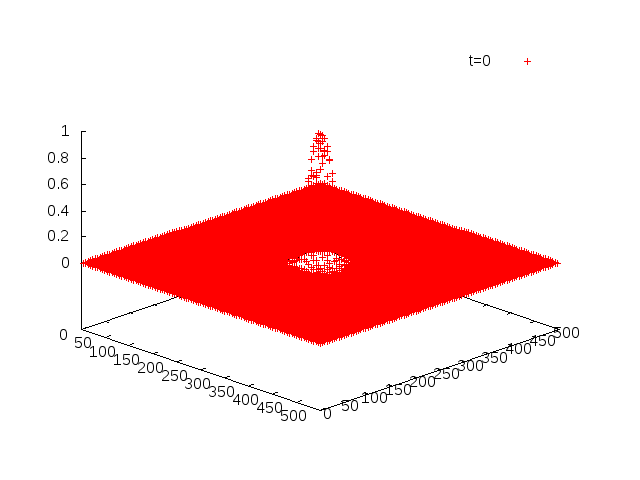
\includegraphics[scale=0.25]{img/anim1-10-1.png}
	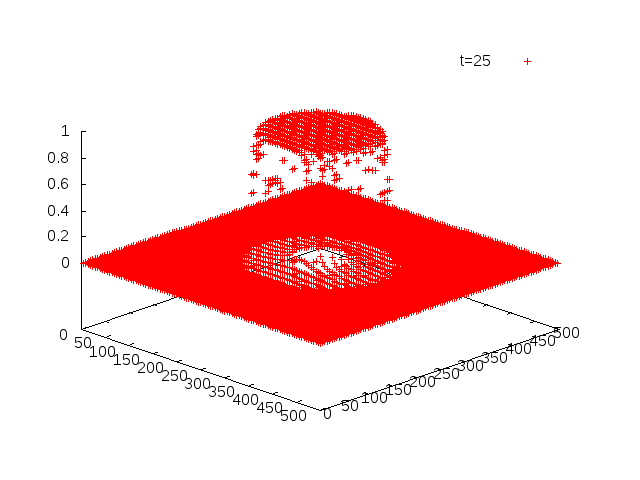
\includegraphics[scale=0.25]{img/anim1-10-50.png}\\
	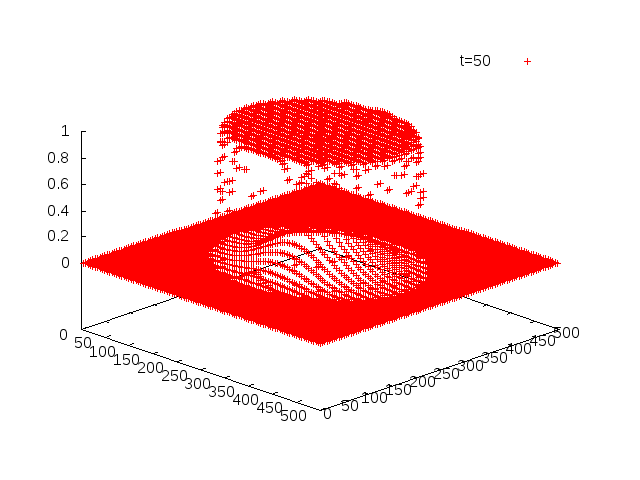
\includegraphics[scale=0.25]{img/anim1-10-100.png}
	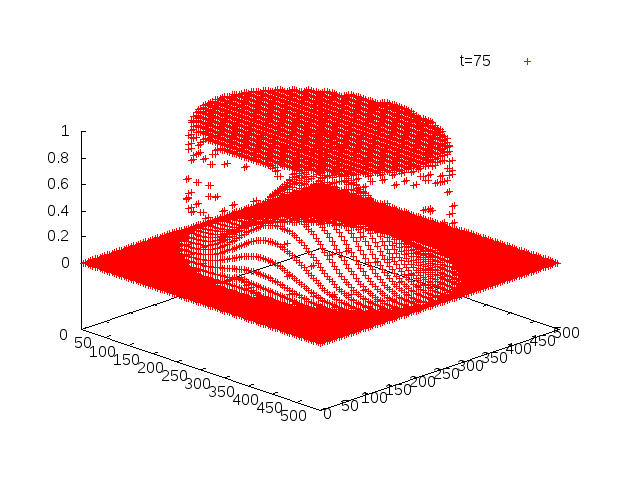
\includegraphics[scale=0.25]{img/anim1-10-150.png}
\caption{Avancée du pathogène : répartition en bande, largeur de 10}
\label{fig1}
\end{figure}

\begin{figure}[!h]
\centering
	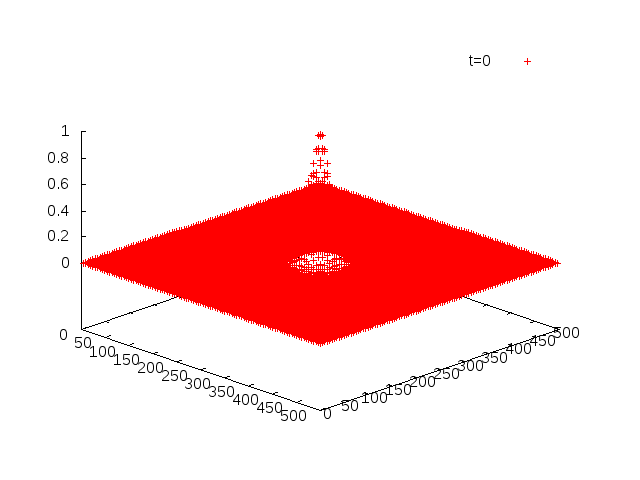
\includegraphics[scale=0.25]{img/anim1-80-1.png}
	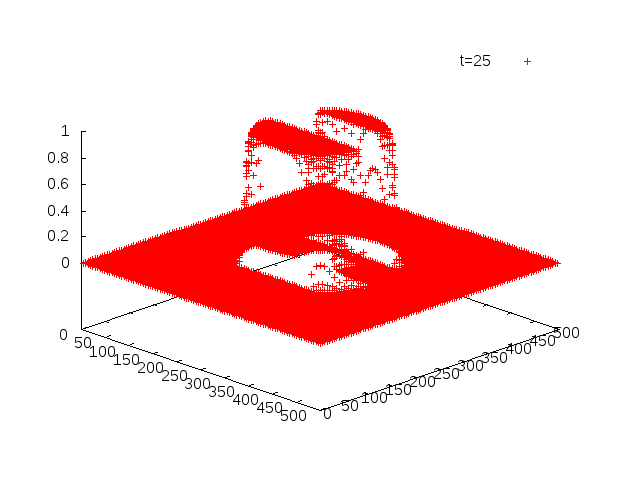
\includegraphics[scale=0.25]{img/anim1-80-50.png}\\
	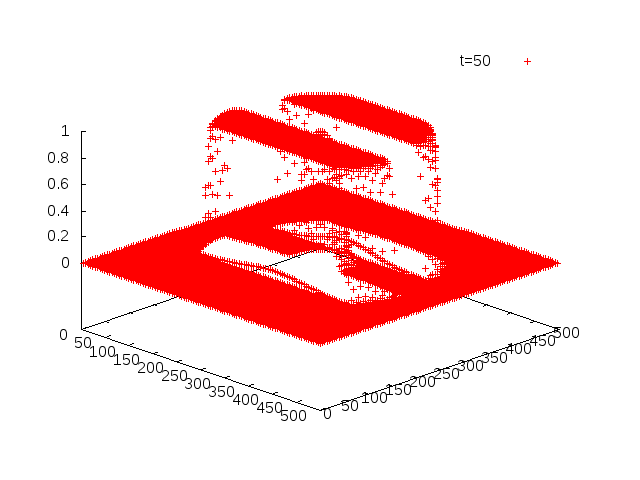
\includegraphics[scale=0.25]{img/anim1-80-100.png}
	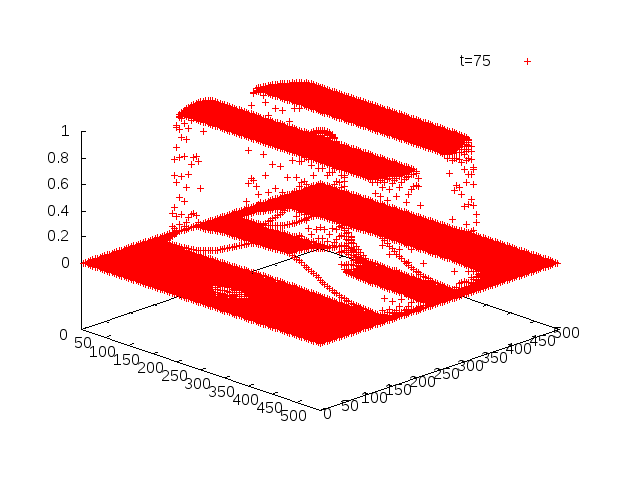
\includegraphics[scale=0.25]{img/anim1-80-150.png}
\caption{Avancée du pathogène : répartition en bande, largeur de 80}
\label{fig2}
\end{figure}

\begin{figure}[!h]
\centering
	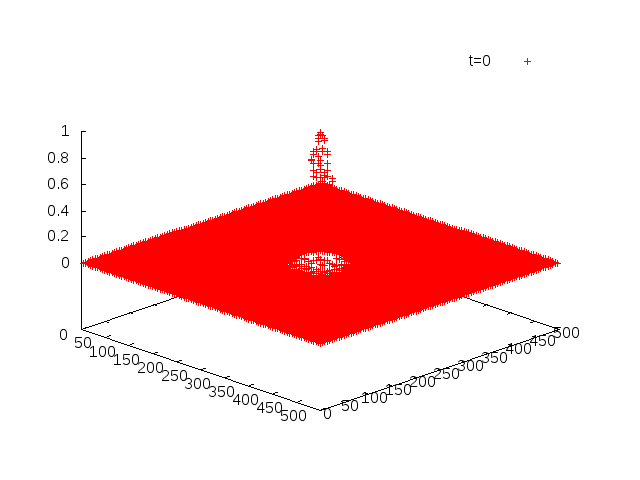
\includegraphics[scale=0.25]{img/anim2-10-1.png}
	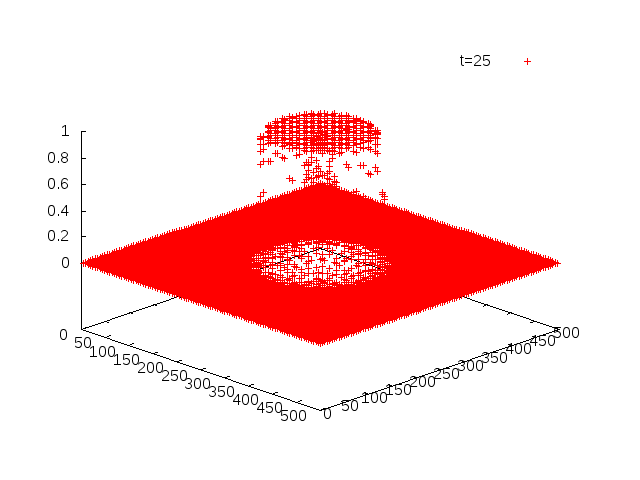
\includegraphics[scale=0.25]{img/anim2-10-50.png}\\
	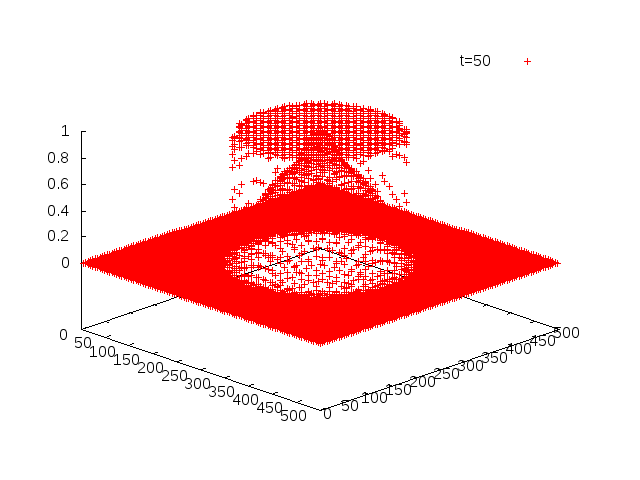
\includegraphics[scale=0.25]{img/anim2-10-100.png}
	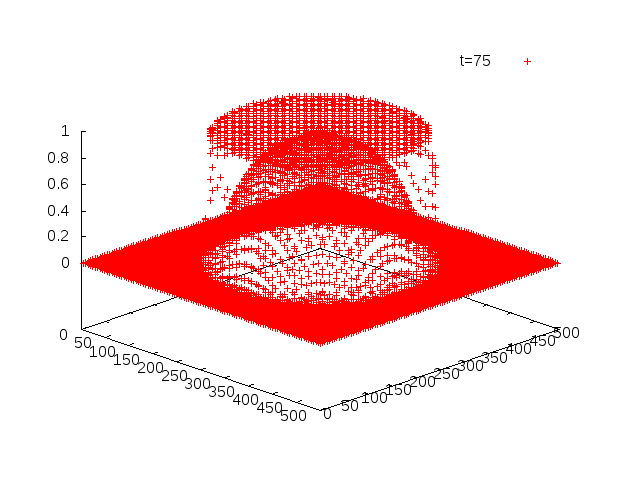
\includegraphics[scale=0.25]{img/anim2-10-150.png}
\caption{Avancée du pathogène : répartition en damier, largeur de 10}
\label{fig3}
\end{figure}

\begin{figure}[!h]
\centering
	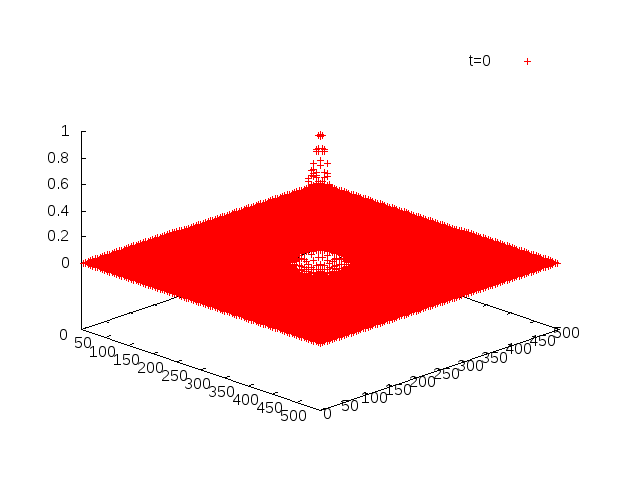
\includegraphics[scale=0.25]{img/anim2-80-1.png}
	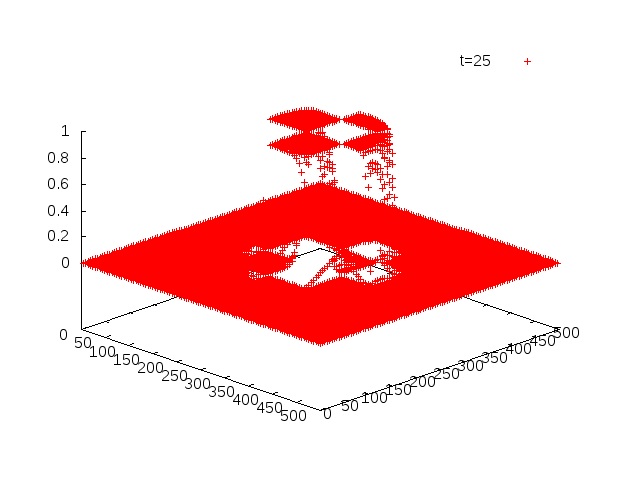
\includegraphics[scale=0.25]{img/anim2-80-50.png}\\
	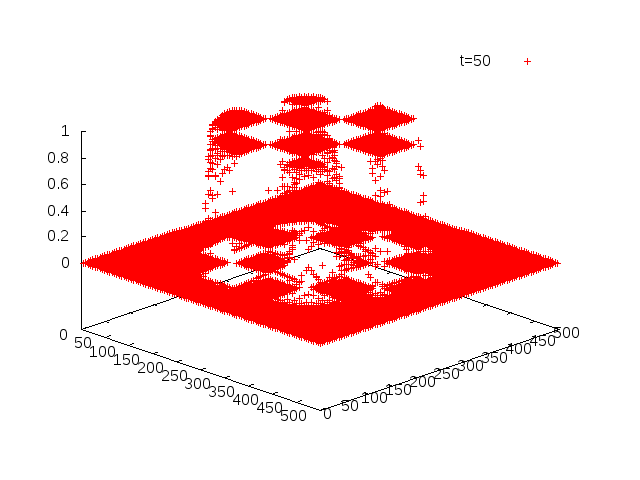
\includegraphics[scale=0.25]{img/anim2-80-100.png}
	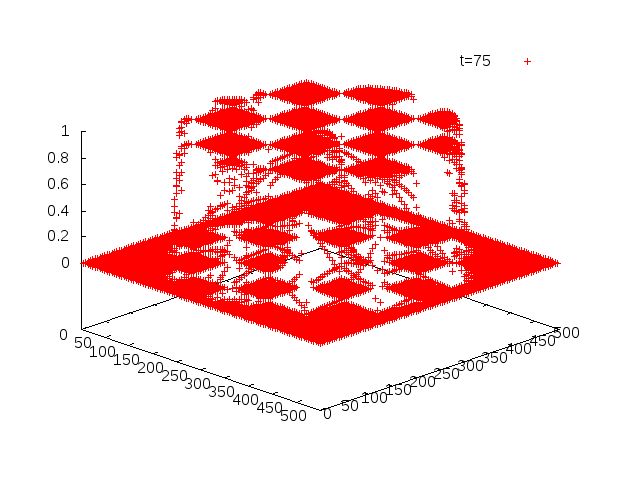
\includegraphics[scale=0.25]{img/anim2-80-150.png}
\caption{Avancée du pathogène : répartition en damier, largeur de 80}
\label{fig4}
\end{figure}

\clearpage
\subsection{Analyse}
Les résultats numériques nous montrent deux choses :
\begin{enumerate}
	\item Même si le taux d'infectés est extrêmement faible sur une bande par exemple, la propagation garde une vitesse très grande sur la bande voisine si la variété présente est plus sensible (voir figure \ref{fig2} par exemple.). Cela rappelle les équations du type équation de Fisher qui présente certaines similitudes.
	\item Selon la répartition des variétés et la largeur des bandes, on remarque que la vitesse de propagation peut grandement changer. Jouer sur ces deux facteurs peut ralentir la propagation d'un pathogène par exemple.
\end{enumerate}
Ceci reste une question clé pour les agronomes. En effet, en plus des différents produits utilisés pour combattre les infections, jouer sur la répartition spatiale des cultures peut également aider à combattre certaines maladies. Mathématiquement, on peut modéliser cela par un problème d'optimisation.\\
Vu sous cet angle, le problème semble simple à résoudre : on ne met que les variétés ayant la plus grande resistance au pathogène et le front sera forcément d'autant plus ralenti. Cependant, certaines contraintes sont à ajouter au problème, comme le fait que toute les variétés doivent être présentent un certain nombre de fois afin d'assurer une certaine biodiversité ou pour avoir une certaine qualité par exemple.

\section{Problème de décision : limiter la propagation du pathogène}
\subsection{Formulation du problème}
Le but est de limiter la propagation du pathogène dans notre domaine ; on va donc chercher une manière de quantifier la propagation de notre maladie dans le champ.\\
La fonction $I(x,t)$ représentant la densité d'infectés au point $x$ à l'instant $t$, on pourrait calculer le nombre d'infectés sur notre domaine (qu'on normalise par la taille du domaine). Si on note $\Omega$ le domaine considéré, notre problème devient :
\begin{equation}\label{pblmOpti}
	\text{Minimiser } \frac{1}{mes(\Omega)}\int_\Omega I(x,t) dx
\end{equation}
Cependant, notre problème est tout de même soumis à des contraintes :
\begin{itemize}
	\item Comme nous l'avons dit dans la section précédente, chaque variété doit être présente un nombre minimal de fois. Ceci peut s'exprimer par exemple en ratio entre l'aire recouverte par la première espèce et l'aire recouverte par la seconde qui doit se trouver entre deux bornes inférieure et supérieure.
	\item Chaque champ doit avoir une taille minimale. En effet, on imagine mal des champs trop fins : ils ne seraient pas exploitables. Ainsi, la largeur des champ aura une borne minimale
	\item Le problème (\ref{pblmOpti}) dépend du temps, et n'est donc pas directement exploitable. De plus, on sait que la propagation sera toujours croissante : on ne traite pas des cas de guérison ou de mort. Ainsi, la propagation atteindra toujours la moitié de la population du domaine, quoi qu'il arrive. On pourrait donc chercher à maximiser le temps $t$ tel que :
	\[\frac{1}{mes(\Omega)}\int_\Omega I(x,t) dx > 0,5\]
\end{itemize}
Sous ces considérations, on arrive donc au problème suivant :
\begin{equation}\label{pblmOptiTot}
\begin{array}{c c}
	\text{Maximiser } &t\\
	\text{tel que } & \left\{\begin{array}{c}
			\frac{1}{mes(\Omega)}\int_\Omega I(x,t) dx > 0,5\\
			r_1\leq R\leq r_2\\
			x_{\mu}>\alpha
			\end{array}\right.
\end{array}
\end{equation}
où $x_{\mu}$ désigne la largeur de bande et $R$ le ratio de présence des deux variétés :
	\[R=\frac{\int_{\Omega} \mathds{1}_{\{\beta(x)=\beta_1\}}(x)dx}{\int_{\Omega} \mathds{1}_{\{\beta(x)=\beta_2\}}(x)dx}\]

Ce problème est très difficilement résolvable : $I$ ne dépendra pas simplement de $t$, et dépend même de $R$ et de $x_{\mu}$ qui seront variables dans ce problème.

\subsection{Techniques d'optimisation}
Le problème n'est pas tellement d'avoir la solution optimale mais au moins une solution assez satisfaisante. Pour cela, il existe plusieurs méthodes d'optimisation basées sur une approche heuristique, comme par exemple le recuit simulé. 

\subsection{Résultats numériques}

\section*{Conclusion}

\bibliographystyle{plain}
\bibliography{pfe}

\end{document}
